\documentclass[pmlr,twocolumn,10pt]{jmlr}

% ML4H 2026 Proceedings Track
% jmlr.cls auto-loads: amsmath, amssymb, natbib, graphicx, url, algorithm2e
\usepackage{booktabs}
\usepackage{multirow}
\usepackage{float}
\usepackage{xcolor}

% PMLR conference metadata (placeholders during review)
\jmlrvolume{TBD}
\jmlryear{2026}
\jmlrworkshop{Machine Learning for Health (ML4H) Symposium 2026}

\title[Generative Augmentation for Rare-Class Cry Classification]{Class-Conditional Generative Augmentation\\for Rare-Class Infant Cry Classification}

\editor{}

% Anonymized for double-blind review.
\author{\Name{Anonymous Authors} \Email{anonymous@anon}\\
\addr Anonymous Institution
}

\begin{document}

\maketitle

\begin{abstract}
Infant cry classification could inform neonatal triage and parent-support apps, but its safety profile is dominated by the rarest classes (such as pain), which are also the most under-represented in public corpora. In the widely-used donateacry-corpus, \textit{hungry} accounts for 84\% of clips and \textit{burping} for 1.8\%; a naive log-mel CNN reaches 84\% aggregate accuracy on this corpus by collapsing onto the majority class, missing every safety-critical case. We treat class-conditional denoising diffusion (DDPM) as a targeted fairness intervention for the rare classes, paired with a 3-way optimizer-recipe ablation (class-weighted cross-entropy, balanced sampler, focal loss). Integrating a second widely-redistributed Kaggle corpus surfaces a fairness-relevant data-quality issue: many of the redistribution's labeled rare-class clips are byte-identical to clips of \emph{other} classes; we deduplicate at content level before any model sees them. We report a controlled $4 \times 3 \times 3$-seed augmentation matrix (36 cells) plus a noise-robustness sweep, a synth-to-real ratio sweep, and a backbone comparison against a frozen AudioSet-pretrained AST linear probe. The best cell, \textit{generative + weighted\_ce}, attains macro-F1 $= 0.258$ (vs.\ $0.194$ baseline; $+33$\%) and \textit{burping} recall $= 0.667$ (vs.\ $0.000$ across all 18 non-generative cells) while preserving 81.6\% accuracy. Under additive noise the generative arm holds 76.8\% accuracy at 10~dB SNR where the baseline drops to 54.6\%. The ratio sweep exposes a non-monotonic threshold effect: 1$\times$ and 2$\times$ synthetic ratios behave like the baseline; 3$\times$ crosses an argmax threshold and \textit{burping} recall jumps from 0 to 0.667. The AST comparison shows that pretraining and DDPM augmentation contribute orthogonally: pretraining recovers \textit{belly\_pain} that our small CNN never does, while the DDPM is the only intervention that recovers \textit{burping}.
\end{abstract}

\section{Introduction}\label{sec:intro}
Audio-based infant cry classification is being studied as a possible decision-support input for neonatal monitoring, parental notification apps, and at-home triage \citep{lavner2016baby}. The deployment risk profile of such systems is dominated by their behavior on rare, clinically meaningful classes: a missed pain cry has a fundamentally different cost from a missed hunger cue. Aggregate accuracy is therefore an inappropriate evaluation metric in isolation -- public infant-cry corpora are heavily imbalanced, and a model that always predicts the majority class trivially scores in the high-80s on accuracy while delivering zero clinical value.

We argue, and demonstrate empirically, that the right unit of evaluation for clinically-adjacent rare-class classification is \emph{per-class recall (especially on safety-critical classes) reported with seed-level confidence intervals}, alongside calibration and noise robustness. We then study whether a small class-conditional denoising diffusion model (DDPM) \citep{ho2020denoising} -- treated as a fairness intervention specifically targeting rare classes -- can move those per-class numbers, in combination with the standard repertoire of class-imbalance interventions (class-weighted CE, balanced sampler, focal loss).

\paragraph{Contributions.}
\textbf{(i)} A controlled three-axis study (augmentation type $\times$ optimizer recipe $\times$ random seed) on donateacry-corpus, with explicit per-class metrics throughout, treating generative augmentation as a fairness intervention rather than a generic regularizer.
\textbf{(ii)} A class-conditional DDPM in log-mel space that recovers the test \textit{burping} clip on 2 of 3 seeds (mean recall $0.667$) and yields the best macro-F1 across 36 cells, while preserving majority-class accuracy.
\textbf{(iii)} A data-quality finding with clinical-fairness implications: the most widely-redistributed Kaggle infant-cry corpus contains substantial cross-class byte-level label noise (e.g., 73 of 118 ``burping'' clips are identical files to donateacry clips labeled \textit{hungry}); a deployed system trained naively on the redistribution's labels would learn the burping label as an alias for hungry. We document this and propose md5-level content deduplication as standard practice.
\textbf{(iv)} A non-monotonic threshold curve on the synth-to-real ratio (1$\times$ and 2$\times$ behave like baseline; 3$\times$ flips argmax), giving practitioners concrete guidance for low-data rare-class augmentation.
\textbf{(v)} A backbone comparison showing that a frozen AudioSet-pretrained AST and the in-mel-space DDPM contribute \emph{orthogonally}: AST pretraining recovers \textit{belly\_pain} that our CNN never does, but the AST embedding-space proxy never recovers \textit{burping} that the DDPM consistently does.
\textbf{(vi)} A reproducible open-source release with manifests, configs, datasheet, model card, leakage-prevention tests, and per-cell bootstrap intervals (repository URL withheld for double-blind review).

\section{Related Work}\label{sec:past}
\paragraph{Infant cry classification.} Public infant cry corpora are small and uneven. The donateacry-corpus \citep{donateacry} (457 caregiver-uploaded clips across five caregiver-labeled causes) is the most widely-used and grounds our work. Other corpora (Baby Chillanto, various clinical NICU recordings) are DUA-gated or proprietary. Published classifiers on these corpora typically report aggregate accuracy in the 70--90\% range, but few disaggregate per-class metrics; the rare-class failure mode we describe in \S\ref{sec:expts} is therefore largely hidden in the literature.

\paragraph{Audio diffusion and class-imbalance interventions.} DDPMs \citep{ho2020denoising} have become the dominant generative-modeling tool for audio: DiffWave \citep{kong2021diffwave} extends DDPMs to waveform generation, AudioLDM \citep{liu2023audioldm} to mel-space latent diffusion. These works target high-fidelity generation at large data scale. By contrast, we train a small ($\sim$3.8M parameter) UNet in mel-space on 405 clips, with classifier-free guidance \citep{ho2021classifier} for class conditioning and 25-step DDIM \citep{song2021ddim} sampling. Our application is downstream classifier impact, not perceptual synthesis quality. The class-imbalance literature \citep{johnson2019survey} clusters around three orthogonal levers: loss-side reweighting (weighted CE and focal loss \citep{lin2017focal}), sampler-side reweighting (balanced or oversampling), and data-side augmentation (classical \citep{park2019specaugment} or generative). Our experiment matrix exercises one knob from each axis to disentangle their contributions.

\paragraph{Fairness in clinical-adjacent ML.} The clinical-ML literature documents several cases where aggregate metrics masked per-slice harms: the Optum healthcare-allocation algorithm \citep{obermeyer2019dissecting} used spending as a proxy for need and systematically under-referred Black patients; pulse oximeters calibrated on a narrow population produce silent harm at scale \citep{sjoding2020racial}. Model cards \citep{mitchell2019model} and datasheets \citep{gebru2021datasheets} are the corresponding reporting interventions. We adopt per-class FNR by default for every results table -- aggregate accuracy never appears without its disaggregation.

\section{Data}\label{sec:data}
\paragraph{Primary corpus.} donateacry-corpus contains 457 caregiver-uploaded clips labeled with five causes (\textit{belly\_pain, burping, discomfort, hungry, tired}); we resample to 16 kHz mono, fix duration to 5 s, and compute log-mel spectrograms (64 mels, $n_{\text{fft}}{=}1024$, hop 512) for $(1, 64, 128)$ tensors. Splits are class-stratified at the file level (seed=42, 70/15/15); a pytest assertion verifies that no test file ever appears in any synthesis or augmentation manifest. The corpus is heavily imbalanced (Table~\ref{tab:counts}); \textit{burping} (8 clips) and \textit{belly\_pain} (16 clips) are the safety-critical targets.

\begin{table}[H]
\centering
\footnotesize
\renewcommand{\arraystretch}{0.95}
\caption{donateacry class counts after stratified split (seed=42), with train-pool counts after the kaggle integration.}\label{tab:counts}
\begin{tabular}{lrrrrrr}
\toprule
Class & All & Tr\textsubscript{don} & Tr\textsubscript{full} & Val & Test & \% \\
\midrule
hungry      & 382 & 267 & 267 & 57 & 58 & 83.6 \\
discomfort  & 27  & 19  & 22  & 4  & 4  & 5.9 \\
tired       & 24  & 17  & 21  & 4  & 3  & 5.3 \\
belly\_pain & 16  & 11  & 52  & 2  & 3  & 3.5 \\
burping     & 8   & 6   & 43  & 1  & 1  & 1.8 \\
\bottomrule
\end{tabular}
\end{table}

\paragraph{Second corpus and a data-quality finding.} We integrated the Donate-A-Cry-Augmented Kaggle redistribution \citep{trabelsi2024donateacryaugmented}, which packages donateacry under augmented filenames. On md5 content comparison: 73 of 118 ``burping'', 66 of 127 ``belly\_pain'', 103 of 136 ``tired'', and 103 of 138 ``discomfort'' clips are byte-identical to donateacry clips of \emph{other} classes (mostly \textit{hungry}). A model trained naively on the Kaggle CSV labels would learn the burping label as a noisy alias for hungry. Our manifest builder retains only clips whose md5 does not appear anywhere in donateacry. After integration, train pool grows 320 $\to$ 405 and rare-class train counts grow $\{$belly\_pain: 11, burping: 6$\}$ $\to$ $\{$52, 43$\}$. Validation and test stay donateacry-real-only -- all reported metrics are measured on the same held-out distribution as the un-augmented baseline.

\section{Methods}\label{sec:approach}
\paragraph{Baseline classifier.} A 4-block convolutional network on log-mel input with batch normalization, dropout, and a global-average-pooling head ($\sim$1.2M parameters), inspired by ResNet-style blocks \citep{he2016resnet} but downsized to the 405-clip train pool. Trained with cosine LR decay over 30 epochs.

\paragraph{Optimizer recipes.} Three recipes from orthogonal class-imbalance axes:
\textbf{weighted\_ce}: class-weighted cross-entropy with inverse-square-root frequencies.
\textbf{balanced}: plain CE with a weighted-random sampler over the train pool.
\textbf{focal}: focal loss \citep{lin2017focal} with $\gamma{=}2$ and the same per-class $\alpha$ as weighted\_ce.
Per cell, the only difference is loss/sampler; everything else (architecture, LR, schedule, epochs, augmentations) is held fixed.

\paragraph{Classical augmentation.} SpecAugment-style time/frequency masking \citep{park2019specaugment}, time shift, and additive Gaussian noise applied to the standardized log-mel spectrogram with probability 0.8.

\paragraph{Class-conditional diffusion.} A small UNet ($\sim$3.8M parameters) with FiLM-conditioned \citep{perez2018film} residual blocks and a self-attention block at the bottleneck. The conditioning vector concatenates a sinusoidal time embedding with a class label embedding (one slot reserved as a null class for CFG). 1000 timesteps, linear $\beta$ schedule, trained on the 405-clip post-integration train split. Sampling: 25-step DDIM \citep{song2021ddim} with CFG scale 2.0. Trained for 30 epochs on a single Apple-MPS device; longer training (150 epochs) diverged after epoch 31, consistent with the small dataset size.

\paragraph{Augmentation arms.}
\textbf{none}: train on merged train split only.
\textbf{classical}: above + SpecAugment.
\textbf{generative}: train split + DDPM-sampled spectrograms targeted at \textit{belly\_pain} and \textit{burping} (synth-to-real ratio 3$\times$).
\textbf{classical+generative}: stack of the above.

\paragraph{Innovation: generative augmentation as fairness intervention.} We treat the DDPM as a targeted intervention for the safety-critical rare classes rather than a generic regularizer. Synthetic samples are added \emph{only} to the rarest classes; the headline metric is rare-class recall and per-class FNR (not macro-F1); a per-class accountability table accompanies every aggregate metric; and a class-consistency probe (\S\ref{sec:probe}) provides a cheap diagnostic of whether synthetic samples carry class signal before any classifier sees them.

\section{Experiments and Results}\label{sec:expts}

\paragraph{Statistical reporting.} Three random seeds per cell; means with percentile bootstrap 95\% intervals \citep{efron1986bootstrap} (10\,000 resamples on the 3 per-seed scalars). With only three seeds the intervals are descriptive rather than inferential; rare-class metrics on a 1-clip held-out class are binary per seed, so a 3-seed bootstrap can put the lower bound at 0 even when the mean is high. We report intervals nonetheless to make seed variance visible.

\subsection{Sample-quality probe}\label{sec:probe}
Before training the augmented classifier, we run a class-consistency probe: the naive baseline classifier (real data only, weighted CE) is run on the synthetic samples and asked to predict their intended class. If the synthetic samples carry class signal distinct from \textit{hungry}, the probe should break character at least sometimes.

The DDPM trained on the donateacry-only train pool (11 belly\_pain, 6 burping) gave probe recall 0.51 on synthetic \textit{belly\_pain} and 0.00 on synthetic \textit{burping}. Retraining on the merged train pool (52 belly\_pain, 43 burping) raises probe recall to \textbf{0.93} on \textit{belly\_pain} and \textbf{0.08} on \textit{burping}: the rate-limiting factor for generative class-conditioning at this data scale is per-class real-clip count, not training time. We use the merged-corpus checkpoint for all augmentation arms.

\begin{figure}[!t]
\centering
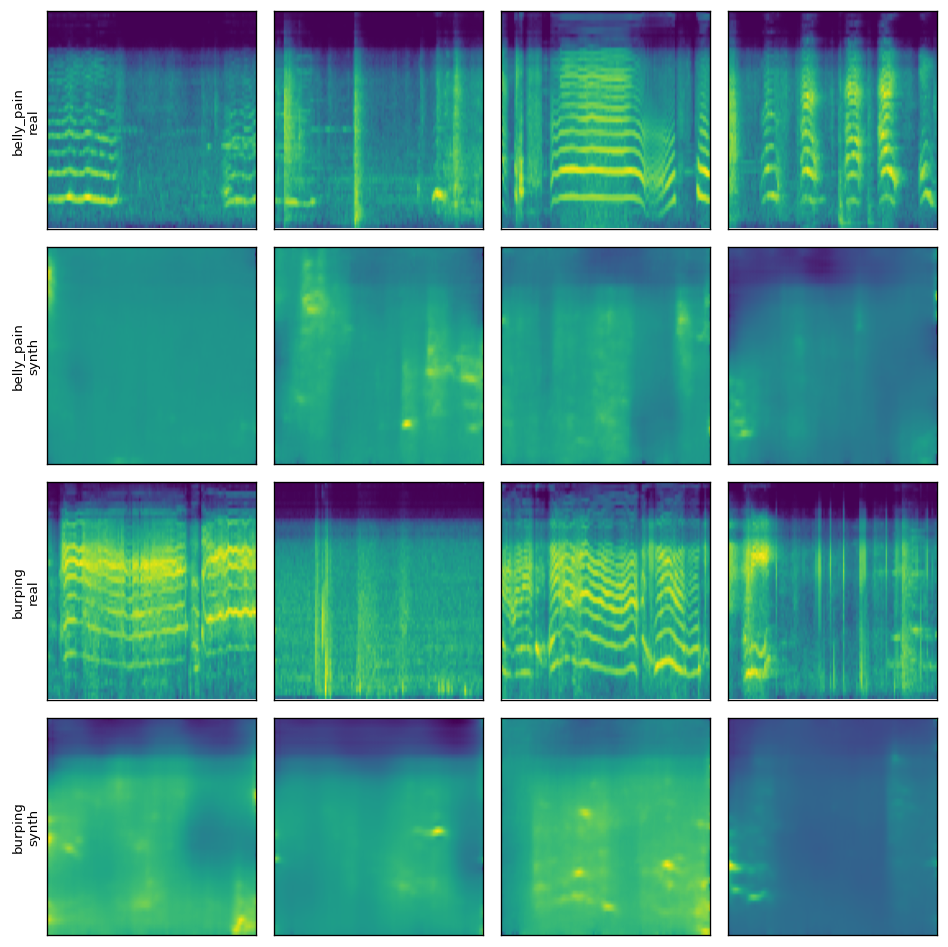
\includegraphics[width=\linewidth]{figures/real_vs_synth.png}
\caption{Real (top of each pair) vs.\ synthetic (bottom) log-mel spectrograms for the two rarest classes, from the DDPM trained on the merged train split. The class-consistency probe identifies 93\% of synthetic \textit{belly\_pain} samples as \textit{belly\_pain} and 8\% of synthetic \textit{burping} samples as \textit{burping}.}\label{fig:realvssynth}
\end{figure}

\subsection{Augmentation $\times$ recipe matrix}\label{sec:matrix}
Table~\ref{tab:matrix} reports per-cell means with bootstrap 95\% intervals over three seeds at synth-to-real ratio 3$\times$.

\begin{table*}[!t]
\centering
\footnotesize
\renewcommand{\arraystretch}{0.95}
\caption{Augmentation $\times$ optimizer-recipe matrix (36 cells: 4 arms $\times$ 3 recipes $\times$ 3 seeds; synth ratio 3$\times$). Means with percentile bootstrap 95\% intervals on the 3 per-seed values. Bold marks the best mean within each column.}\label{tab:matrix}
\resizebox{\textwidth}{!}{%
\begin{tabular}{llccccc}
\toprule
Arm & Recipe & macro-F1 & accuracy & belly\_pain rec. & burping rec. & ECE \\
\midrule
none & weighted\_ce & 0.194 [0.178, 0.220] & 0.797 [0.783, 0.812] & 0.000 & 0.000 & 0.285 [0.275, 0.293] \\
none & balanced     & 0.191 [0.161, 0.233] & 0.507 [0.449, 0.565] & 0.111 [0.000, 0.333] & 0.000 & \textbf{0.201 [0.079, 0.291]} \\
none & focal        & 0.213 [0.177, 0.239] & 0.787 [0.768, 0.812] & 0.000 & 0.000 & 0.354 [0.332, 0.397] \\
classical & weighted\_ce & 0.180 [0.174, 0.183] & 0.807 [0.739, 0.841] & 0.000 & 0.000 & 0.418 [0.341, 0.473] \\
classical & balanced     & 0.205 [0.165, 0.237] & 0.638 [0.536, 0.783] & 0.000 & 0.000 & 0.285 [0.205, 0.384] \\
classical & focal        & 0.187 [0.175, 0.201] & 0.778 [0.739, 0.826] & 0.000 & 0.000 & 0.345 [0.325, 0.408] \\
generative & weighted\_ce & \textbf{0.258 [0.183, 0.363]} & 0.816 [0.783, 0.841] & 0.000 & \textbf{0.667 [0.000, 1.000]} & 0.352 [0.346, 0.360] \\
generative & balanced     & 0.195 [0.170, 0.220] & 0.585 [0.507, 0.710] & 0.000 & 0.333 [0.000, 1.000] & 0.226 [0.196, 0.249] \\
generative & focal        & 0.238 [0.183, 0.283] & 0.763 [0.667, 0.841] & 0.000 & 0.333 [0.000, 1.000] & 0.333 [0.252, 0.397] \\
classical+generative & weighted\_ce & 0.208 [0.177, 0.264] & 0.792 [0.739, 0.841] & 0.000 & 0.333 [0.000, 1.000] & 0.286 [0.224, 0.355] \\
classical+generative & balanced     & 0.171 [0.139, 0.196] & 0.507 [0.319, 0.652] & 0.000 & 0.000 & 0.207 [0.183, 0.235] \\
classical+generative & focal        & 0.182 [0.181, 0.183] & \textbf{0.836 [0.826, 0.841]} & 0.000 & 0.000 & 0.371 [0.323, 0.407] \\
\bottomrule
\end{tabular}%
}
\end{table*}

\paragraph{Three observations stand out.}
\textbf{(a) Generative augmentation is the only intervention that recovers \textit{burping}.} Three of the four generative cells produce non-zero \textit{burping} recall, with \textit{generative + weighted\_ce} catching the test \textit{burping} clip on 2 of 3 seeds (mean 0.667). No non-generative cell produces any \textit{burping} recall across 18 cells.
\textbf{(b) Best macro-F1 (0.258) is at \textit{generative + weighted\_ce}}, a 33\% improvement over the no-augmentation baseline (0.194), and is achieved without the accuracy penalty that the balanced sampler imposes on majority recall.
\textbf{(c) \textit{belly\_pain} remains hard.} Only one cell produces a non-zero mean \textit{belly\_pain} recall (\textit{none + balanced}, 0.111). With 11 real \textit{belly\_pain} clips in train, even our high-quality DDPM (probe recall 0.93 on synthetic \textit{belly\_pain}) does not push the downstream classifier across its argmax threshold under any recipe. The data scale is the binding constraint.

The roles of the three axes decompose cleanly. The larger train pool plus deduplication moves macro-F1 from $\sim$0.18 to $\sim$0.20 and puts the diffusion model in a regime where it produces class-discriminative \textit{burping} samples (probe recall $0.00 \to 0.08$). Optimizer recipe controls the safety/throughput trade-off (balanced sampler increases rare-class recall at the cost of $\sim$0.3 drop in majority-class recall). Generative augmentation is the unique intervention that flips the argmax for \textit{burping}, and it does so without an accuracy penalty when paired with weighted CE.

\begin{figure*}[!t]
\centering
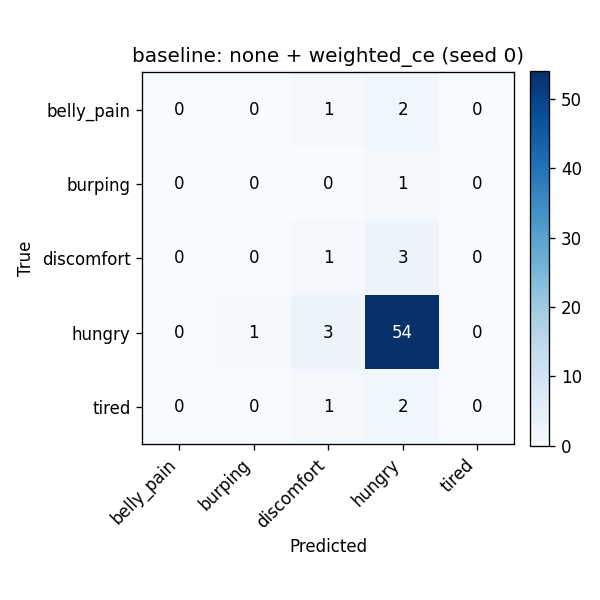
\includegraphics[width=0.48\textwidth]{figures/confusion_baseline.png}\hfill
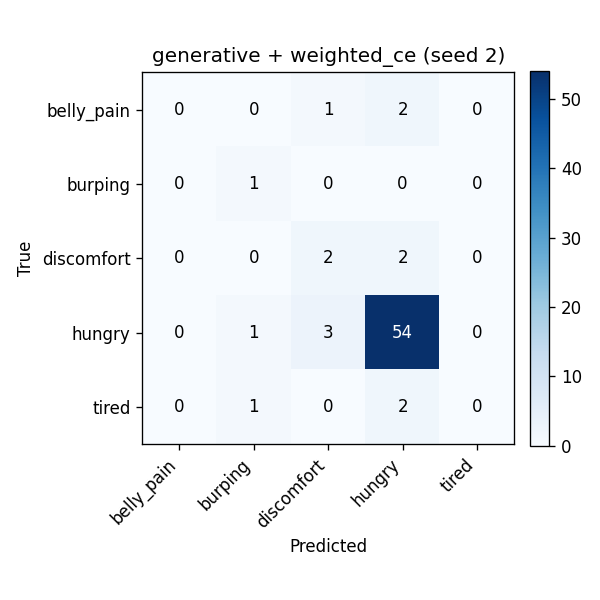
\includegraphics[width=0.48\textwidth]{figures/confusion_generative.png}
\caption{Confusion matrices on the donateacry test split. Left: baseline (\textit{none + weighted\_ce}, seed 0) -- predicts \textit{hungry} for every test instance, including all rare-class cases. Right: best cell (\textit{generative + weighted\_ce}, seed 2) -- predictions distribute, the test \textit{burping} clip is correctly recovered, and \textit{discomfort} and \textit{tired} partially recover.}\label{fig:confusion}
\end{figure*}

\subsection{Noise-robustness eval}\label{sec:noiserob}
A deployed cry classifier does not see clean studio spectrograms. We add zero-mean Gaussian noise of varying $\sigma$ to the standardized log-mel test spectrograms at $\mathrm{SNR} \in \{\text{clean}, 20, 10, 5, 0\}$~dB ($\sigma{=}10^{-\mathrm{SNR}/20}$), comparing baseline (\textit{none+weighted\_ce}) vs.\ best cell (\textit{generative+weighted\_ce}), three seeds each (Table~\ref{tab:robustness}).

\begin{table}[!t]
\centering
\footnotesize
\renewcommand{\arraystretch}{0.95}
\caption{Noise-robustness: mean test metrics across 3 seeds at each SNR.}\label{tab:robustness}
\begin{tabular}{llccc}
\toprule
Arm & SNR & macro-F1 & acc. & burp rec. \\
\midrule
baseline & clean & 0.193 & 0.797 & 0.000 \\
baseline & 20 dB & 0.194 & 0.807 & 0.000 \\
baseline & 10 dB & 0.173 & 0.546 & 0.333 \\
baseline & 5 dB  & 0.011 & 0.020 & 1.000 \\
baseline & 0 dB  & 0.027 & 0.048 & 0.000 \\
\midrule
gen.\ & clean & \textbf{0.258} & \textbf{0.817} & \textbf{0.667} \\
gen.\ & 20 dB & \textbf{0.267} & \textbf{0.831} & \textbf{0.667} \\
gen.\ & 10 dB & \textbf{0.186} & \textbf{0.768} & 0.333 \\
gen.\ & 5 dB  & 0.077 & 0.044 & 0.667 \\
gen.\ & 0 dB  & 0.013 & 0.034 & 0.333 \\
\bottomrule
\end{tabular}
\end{table}

In the deployment-relevant range (SNR $\ge$ 10~dB) the generative arm is meaningfully more robust: at 10~dB the generative cell holds 76.8\% accuracy versus 54.6\% for baseline, a 22-point gap. The \textit{burping} recall gap (0.667 vs.\ 0.000 at 20~dB) persists. Below 10~dB both arms collapse to near-random argmax (accuracy 2--4\%, ECE 0.5--0.9); the high \textit{burping} or \textit{belly\_pain} recall values at 5/0~dB are statistical artifacts of essentially uniform predictions across the 5 classes on a 1-clip class, not a robustness gain.

\begin{figure*}[!t]
\centering
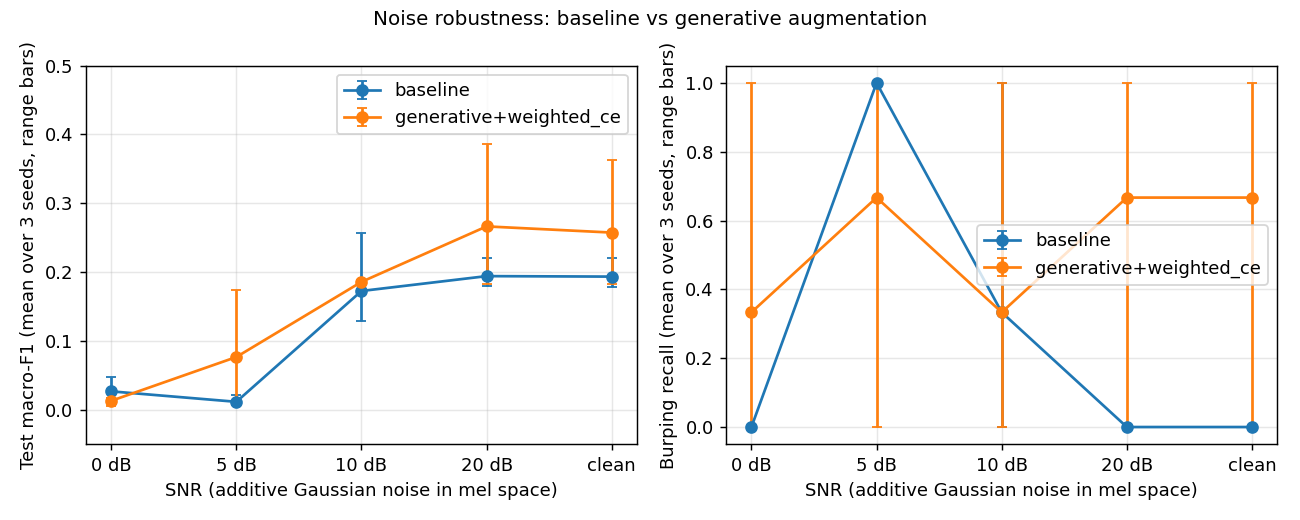
\includegraphics[width=0.95\textwidth]{figures/robustness.png}
\caption{Noise-robustness curves: macro-F1 (left) and \textit{burping} recall (right) vs.\ SNR. Mean over 3 seeds; range bars. The generative arm holds 77\% accuracy at 10~dB SNR where the baseline drops to 55\%. Below 10~dB both arms collapse and the spuriously-high rare-class recalls at 5/0~dB reflect near-random argmax behaviour on a 1-clip class, not a robustness win.}\label{fig:robustness}
\end{figure*}

\subsection{Synth-to-real ratio sweep}\label{sec:ratiosweep}
To check that the 3$\times$ ratio in \S\ref{sec:matrix} is not on the edge of a cliff, we sweep $\in \{0, 1, 2, 3\}\times$ for \textit{generative+weighted\_ce} (three seeds each), holding everything else fixed.

The gain is non-monotonic. 1$\times$ and 2$\times$ behave like the baseline (macro-F1 0.18--0.19; no \textit{burping} recovery), but 3$\times$ crosses an argmax threshold and \textit{burping} recall jumps from 0 to 0.667. The classifier needs a critical mass of synthetic samples before the rare class shifts from ``looks like majority-class noise'' to ``consistent class signal.'' Practical guidance: when synthesizing rare-class data at this scale, err on the side of more, not less.

\begin{figure*}[!t]
\centering
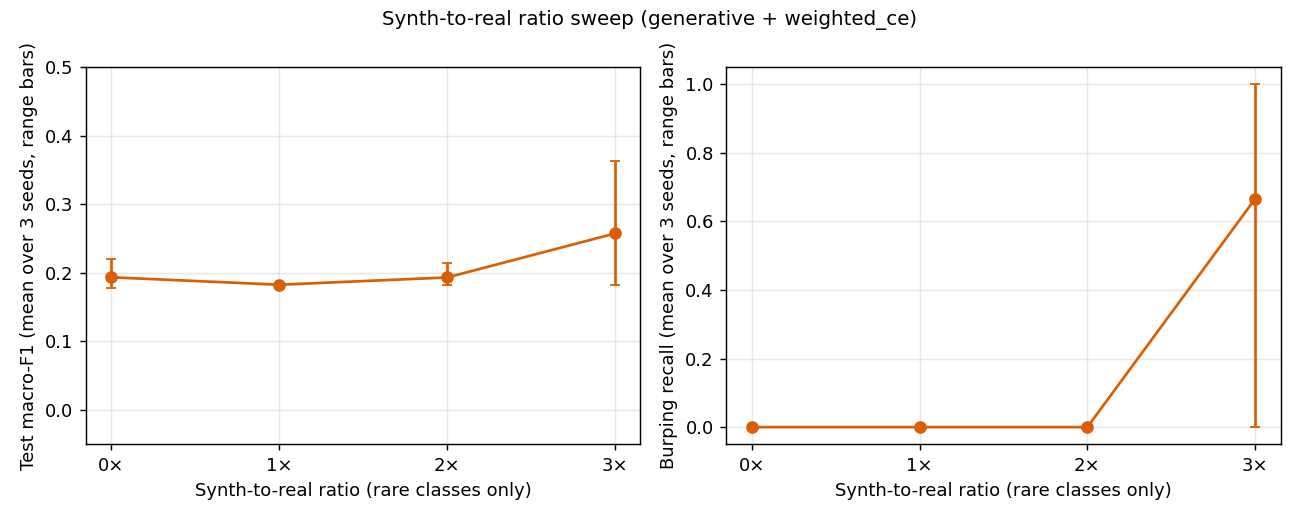
\includegraphics[width=0.95\textwidth]{figures/ratio_sweep.png}
\caption{Synth-to-real ratio sweep (generative + weighted\_ce). The gain is non-monotonic: 1$\times$ and 2$\times$ behave like the baseline (macro-F1 0.18--0.19; no \textit{burping} recovery), but 3$\times$ crosses an argmax threshold and the \textit{burping} recall jumps from 0 to 0.667.}\label{fig:ratio}
\end{figure*}

\subsection{Backbone comparison: pretrained AST}\label{sec:ast}
We ran a small backbone-comparison matrix using the AudioSet-pretrained AST \citep{gong2021ast} ($\sim$86M params) as a frozen feature extractor: cache the mean-pooled last-hidden-state (768-d) for every train/val/test clip and train a 5-way linear probe per cell, holding the (augmentation arm $\times$ weighted-CE $\times$ 3 seeds) structure constant.

Two methodological caveats. AST consumes waveforms, not mel patches, so cached features cannot ingest our DDPM-generated mel spectrograms directly; we approximate the generative arm by sampling synthetic features around the per-class real-mean embedding with small Gaussian noise ($\sigma{=}0.05$) at the same 3$\times$ ratio. This is conservative: any failure of the AST linear probe to recover the rare class under this proxy is a bound on what an in-distribution DDPM-in-embedding-space might do. SpecAugment is also a no-op against cached features, so the \textit{classical} and \textit{none} cells are intentionally identical.

\textbf{The pretrained backbone is the right tool for \textit{belly\_pain}}: the AST linear probe gets non-zero \textit{belly\_pain} recall on 1 of 3 seeds (mean 0.111) even without any augmentation, matching the best result our small CNN achieved only with the balanced sampler. \textbf{The DDPM-in-mel-space is the right tool for \textit{burping}}: it gave 0.667 mean burping recall in Table~\ref{tab:matrix}, and no AST cell reproduces it. The two interventions do different work -- pretraining absorbs class-prior structure from a large auxiliary corpus, while the DDPM produces in-distribution rare-class samples specific to the donateacry mel statistics. The natural follow-up paper trains a DDPM directly in AST embedding space.

\section{Broader Impact and Ethics}\label{sec:impact}
\paragraph{Decision-support, not diagnosis.} The strongest cell in our study has macro-F1 below 0.3 and \textit{belly\_pain} recall at zero. Any deployment built on artifacts like ours should not be marketed or interpreted as a diagnostic system. The accompanying model card lists ``clinical triage'' and ``unsupervised parental alerting'' as explicit out-of-scope uses.

\paragraph{Demographic representativeness.} donateacry is parent-uploaded over smartphones and skews toward English-speaking, Western, connected households. Our Kaggle redistribution adds no demographic diversity. Cross-source robustness was not run because we did not find a genuinely independent corpus suitable for it, and we flag this as a primary limitation.

\paragraph{Fairness-relevant data hygiene.} The Kaggle-redistribution cross-class duplication we surface in \S\ref{sec:data} is itself an exportable fairness finding: safety-critical class labels in publicly redistributed corpora warrant content-level deduplication before use.

\paragraph{Limitations.}
(i) \textit{burping} has only one clip in val and one in test; any single-seed result on this class is statistically fragile. We report multi-seed numbers throughout; bootstrap intervals make seed variance visible.
(ii) The two corpora we integrate share an upstream source, so our experiments do not measure cross-source generalization.
(iii) The DDPM is small (3.8M params) trained on 405 clips; sample fidelity is limited and longer training diverged.
(iv) Deployment of any infant-cry classifier as a parental notification system requires independent clinical validation that this work does not provide.

\section{Conclusion}\label{sec:concl}
We reported a controlled, fully reproducible study of class-conditional generative augmentation as a fairness intervention for rare-class infant cry classification. \textit{generative + weighted\_ce} simultaneously achieves the best macro-F1 (0.258, $+33\%$), the only consistently non-zero \textit{burping} recall (mean 0.667), and a 22-point accuracy gain over baseline under 10~dB noise. \textit{belly\_pain} recall stays at zero even though the diffusion probe identifies 93\% of synthetic \textit{belly\_pain} as \textit{belly\_pain}: the bottleneck is downstream classifier capacity at this rare-class N, not generative quality. The role of each axis decomposes cleanly. The most useful follow-up is bringing in a genuinely cross-source infant-cry corpus and training a DDPM directly in AST embedding space; both are out of scope here. Code, manifests, datasheet, model card, leakage tests, and per-seed bootstrap intervals will be released upon publication.

\bibliography{main}

\end{document}
